\documentclass[12pt]{report}
\usepackage[print,nopanel]{pdfscreen}
\begin{print}
\usepackage{lipsum}% http://ctan.org/pkg/lipsum
\usepackage{titletoc}% http://ctan.org/pkg/titletoc
\usepackage{lastpage}
\usepackage{macro/macro}
\usepackage{float}
\usepackage{wrapfig}
\usepackage{fancyhdr}
\usepackage{verbatim}
%Options: Sonny, Lenny, Glenn, Conny, Rejne, Bjarne, Bjornstrup
\usepackage[Glenn]{fncychap}
\lhead{\large\bfseries Elearning System}
\usepackage[left=2.5cm, right=1.5cm, top=2.5cm, bottom=1.5cm]{geometry}
\pagestyle{fancy}
\end{print}
\margins{.5cm}{.5cm}{.5cm}{.5cm}
\begin{screen}

\renewcommand{\encodingdefault}{T1}
\usepackage{setspace}
\linespread{1.5}
\renewcommand{\rmdefault}{ptm}
\end{screen}
\screensize{8cm}{9cm}
\overlay{overlay8.pdf}
\usepackage{graphicx}

\begin{document}
\newcommand{\centertext}[1]{\begin{center}\textbf{#1}\end{center}}
\newcommand{\student}{\vskip 2.5cm}
\newcommand{\supervisor}{\vskip 2cm}
\newcommand{\stamp}{\vskip 2.5cm}
\newcommand{\HRule}{\rule{\linewidth}{0.5mm}}
\newcommand{\projecttitle}{\Huge \bf{Elearning System}\vskip 0.5in}
\newcommand{\tab}[1]{\hspace{.4\textwidth}\rlap{#1}}
\newcommand{\itab}[1]{\hspace{.05\textwidth}\rlap{#1}}
\newcommand{\logo}[1]{\includegraphics[scale=0.7]{#1}}
\newcommand{\submitted}{
\vskip 0.4in
\textnormal{Submitted for partial fulfilment of the Degree\\
of\\
Bachelor of Technology\\
(Computer Science and Engineering)\\
}
\vskip 2.5cm
%\image{0.7}{images/gne.jpg}{}
\logo{images/gne.jpg}
\vskip 3.0cm
\begin{minipage}{0.4\textwidth}
\begin{flushleft} \large
{Submitted By:}\\
\textnormal{Navdeep Singh\\
1243678} % Your name
\end{flushleft}
\end{minipage}
~
\begin{minipage}{0.4\textwidth}
\begin{flushright} \large
{Submitted To:} \\
\textnormal{Sukhjit Singh Sehra\\                                                                                                                          
CSE Department} % Supervisor's Name
\end{flushright}
\end{minipage}\\[2cm]
\HRule \\[0.4cm]

\textnormal{Department of Computer Science \& Engineering \\
Guru Nanak Dev Engineering College \\
Ludhiana 141006}
}


\newcommand{\pagetitle}{\begin{center}
\projecttitle
\Large\textbf{Project Report}\\
\submitted
\vskip 1cm

\end{center}}
\newcommand{\openoffice}{\textbf{OpenOffice}}
\newcommand{\frontmatter}[1]{\begin{Large} \textbf{#1} \end{Large}}
\newcommand{\ppttitle}{\begin{center}
\end{center}}


\begin{screen}
\ppttitle
\end{screen}
\footskip 0.7cm
\thispagestyle{empty} 
\pagetitle
\newpage
\pagenumbering{Roman}
\cfoot{\thepage}

\begin{Large}
\centertext{Acknowledgement}
\end{Large}
The author is highly grateful to Dr. M.S. Saini Director, Guru
Nanak Dev Engineering College Ludhiana for providing this
opportunity to carry out the six month industrial training at	 APTECH Ludhiana.\\

\noindent The constant guidance and encouragement received from Dr. K. S. Mann Dean T\&P, has been of great help in carrying out the project work and is acknowledged 
with reverential thanks.\\

\noindent The author would like to express a deep sense of gratitude and thanks profusely to Mrs. Nitu Verma Centre Head of APTECH. Without her wise counsel and able guidance, it would have been impossible to complete the report in this manner.\\

\noindent The author expresses gratitude to other faculty members of CSE department 
of GNDEC for their intellectual support throughout the course of this 
work.\\

\noindent Finally, the author is indebted to all whosoever have contributed in
this report work Gurjot Pal Singh (D4 CSE) and all other classmates. Without their 
encouragement, it would not have been possible to complete this project
in such an efficient manner.

\vskip 1.0cm 
\noindent Navdeep Singh

\newpage

\begin{Large}
\centertext{Abstract}
\end{Large}
‘E-learning comprises all forms of electronically supported learning and teaching. The information and communication systems, whether networked learning or not, serve as specific media to implement the learning process. The term will still most likely be utilized to reference out-of-classroom and in-classroom educational experiences via technology, even as advances continue in regard to devices and curriculum.\\

\noindent Elearning was made keeping in mind that the various schools and colleges who spend several man hours, which often run into days, giving students assignments and other class related work. This project will not only help them significantly reduce the time consumed in giving the assignments and other class related work, but will also make the overall process very simple and easy to use.\\

\noindent The motive of the project is to reduce the time consumed and to enable fast and
easy customization and even faster processing of class work when required as instead of writing and
scaling, only values in the php script need to be changed.\\

\noindent Also, this project is completely open source and is made using HTML, CSS, PHP and MySql and the entire code is available to the user as and when required. There is also a Complete Documentation as well as User manual alongwith it for making the 
developing and using the software a lot easier.


\newpage
\tableofcontents
\newpage
\listoffigures
\newpage

\pagenumbering{arabic}
\cfoot{\thepage}

\newpage
\chapter{Introduction To Organisation}
\begin{figure}[ht]
\centering
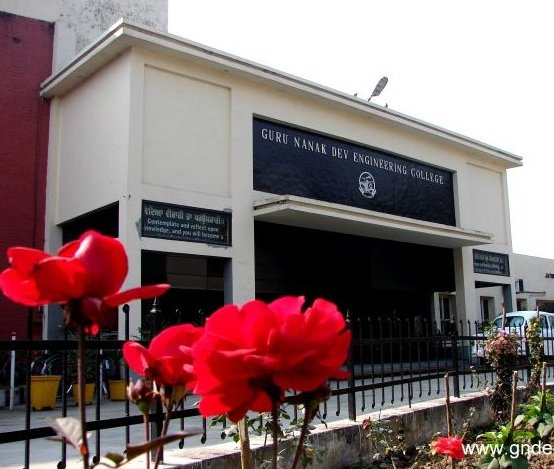
\includegraphics[scale=0.7]{images/gndec.jpg}
\caption{Guru Nanak Dev Engineering College}
\end{figure}
\hspace{-1.7em} I had my Six Month Industrial Training at APTECH Ludhiana. Guru Nanak Dev Engineering College was established by the Nankana
Sahib Education Trust Ludhiana. The Nankana Sahib Education Trust i.e NSET
was founded in memory of the most sacred temple of Sri Nankana Sahib, birth place
of Sri Guru Nanak Dev Ji. With the mission of Removal of Economic Backwardness
through Technology Shiromani Gurudwara Parbandhak Committee i.e SGPC started a
Poly technical was started in 1953 and Guru Nanak Dev Engineering College was established in 1956.\\\\
NSET resolved to uplift Rural areas by admitting 70\% 
of students from these rural
areas ever year. This commitment was made to nation on 8th April, 1956, the day
foundation stone of the college building was laid by Dr. Rajendra Prasad Ji, the First
President of India. The College is now ISO 9001:2000 certified.\\\\
Guru Nanak Dev Engineering College campus is spread over 88 acres of prime land
about 5 Km s from Bus Stand and 8 Km s from Ludhiana Railway Station on Ludhiana-Malerkotla Road. The college campus is well planned with beautifully laid out tree plantation, pathways, flowerbeds besides the well maintained sprawling lawns all around. It
has beautiful building for College,Hostels,Swimming Pool,Sports and Gymnasium Hall
Complex, Gurudwara Sahib, Bank, Dispensary, Post Office etc. There are two hostels
for boys and one for girls with total accommodation of about 550 students. The main
goal of this institute is:\\\\
\begin{itemize}
\item To build and promote teams of experts in the upcoming specialisations.
\item To promote quality research and undertake research projects keeping in view their
relevance to needs and requirements of technology in local industry.
\item To achieve total financial independence.
\item To start online transfer of knowledge in appropriate technology by means of establishing multipurpose resource centres.
\end{itemize}
\section{APTECH Ludhiana}
My Six Month Industrial Training was done by me at APTECH Ludhiana under the guidance of Mrs. Ritu Verma Centre Head Aptech Ludhiana. 

\begin{figure}[ht]
\centering

\includegraphics[scale=0.9]{images/Aptech.jpg}
\caption{Aptech Computer Education}
\end{figure} 

\noindent Aptech Computer Education is a premier IT
education Institute. Established in 1986, Aptech is a
pioneer in IT software \& hardware training. The Institute has successfully trained more than 70
lakh (7 million) students through its wide network
of education centres located in over 40 countries.\\

\noindent Aptech offers a variety of courses - technology
courses for IT students, career programs for students
wanting to enter the IT sector, certification courses
for IT professionals to enhance their career and basic
IT programs for school students, housewives/senior
citizens etc. Class timings are such that even working people can attend courses as per their convenience.\\

\noindent Aptech Computer Education has alliances with three of the leading computer technology companies to offer courses that are globally recognized. These tie-ups enable us to provide our students official curriculum of international standards. In addition, students also receive discounts on certification exams and a participation certificate by the respective global alliance partners. Aptech Computer Education prepares students to be a part of this growing industry through its
courses, partnerships with technology companies like Microsoft, Red Hat, Oracle \& various placement assistance activities.\\\\


THE ACADEMY OFFERS:\\
\begin{itemize}
\item World class quality of education.
\item A wide range of courses.
\item Benefits through partnerships with leading technology companies such as Microsoft, Red Hat, Java \& Oracle.
\item Job placement assistance after successful completion of career courses
\end{itemize}


\newpage
\chapter{\LaTeX}
\section{Introduction to \LaTeX}

\LaTeX, I have used this tool for preparing my six weeks training report and i found it excellent. So this time again i decided to use it for my report.
\LaTeX{} (pronounced /ˈleɪtɛk/, /ˈleɪtɛx/, /ˈlɑːtɛx/, or /ˈlɑːtɛk/) is a 
document markup language and document preparation system for the \TeX{} 
typesetting  program. Within the typesetting system, its name is styled 
as \LaTeX.

\image{0.9}{images/donald.png}{Donald Knuth, Inventor Of \TeX{} 
typesetting system}

\noindent Within the typesetting system, its name is styled as \LaTeX. The term 
\LaTeX{} refers only to the language in which documents are written, 
not to the editor used to write those documents. In order to create a 
document in \LaTeX, a .tex file must be created using some form of text 
editor. While most text editors can be used to create a \LaTeX{} document, 
a number of editors have been created specifically for working with \LaTeX.

\noindent \LaTeX{} is most widely used by mathematicians, scientists, 
engineers, philosophers, linguists, economists and other scholars in 
academia. As a primary or intermediate format, e.g., translating DocBook 
and other XML-based formats to PDF, \LaTeX{} is used because of the 
high quality of typesetting achievable by \TeX. The typesetting system 
offers programmable desktop publishing features and extensive facilities 
for automating most aspects of typesetting and desktop publishing, 
including numbering and cross-referencing, tables and figures, 
page layout and bibliographies.

\noindent \LaTeX{} is intended to provide a high-level language that
accesses the power of \TeX. \LaTeX{} essentially comprises a
collection of \TeX{} macros and a program to process \LaTeX documents. 
Because the \TeX{} formatting commands are very low-level, it is usually 
much simpler for end-users to use \LaTeX{}.


\section{Typesetting}
\LaTeX{} is based on the idea that authors should be able to focus on 
the content of what they are writing without being distracted by its 
visual presentation. In preparing a \LaTeX{} document, the author 
specifies the logical structure using familiar concepts such as 
chapter, section, table, figure, etc., and lets the \LaTeX{} system 
worry about the presentation of these structures. It therefore 
encourages the separation of layout from content while still allowing 
manual typesetting adjustments where needed. 

\begin{verbatim}
\documentclass[12pt]{article}
\usepackage{amsmath}
\title{\LaTeX}
\date{}
\begin{document}
  \maketitle 
  \LaTeX{} is a document preparation system 
  for the \TeX{} typesetting program.
   \par 
   $E=mc^2$
\end{document}
\end{verbatim}


\chapter{Introduction To Project}
\section{Overview}
E-learning refers to using electronic applications and processes to learn. e-learning applications and processes include Web-based learning, computer-based learning, virtual classrooms and digital collaboration. Elearning is learning utilizing electronic technologies to access educational curriculum outside of a traditional classroom. Elearning is intended to provide features which make it possible to simplify, improve,
and automate the daily class work or activities of a school or college.\\

\noindent Elearning is intended to provide methods or solutions to help our teachers as well as students to improve internal processes, save time and increase efficiency. 
Elearning is all about using the computer to:
\begin{itemize}
\item Make your work less tedious.
\item Trim hours of your workload.
\item Keeping track of all the work done by students.
\item Reduce the Carbon Footprint.
\item To reduce the travel time and cost.
\item Enhance the computer and internet skills.
\end{itemize}
The use of computer systems to execute a variety of operations, such as adding downloadable material,
online quiz and tests, uploading and giving grades for assignments through internet refers to what we call Elearning. The flexible nature of elearning means that we are likely to encounter it in everyday life. Some people seek it out in for additional learning opportunities, and for career advancement. While others may accidentally stumble upon it when watching a short training on their smartphone about their latest application. The old adage still rings true, and e-Learning brings with it new dimensions in education.

\section{The Existing System}
Existing system is manual system where there is no role of computer. 
People use pen, paper to make records and consignment notes.\\

\noindent{\bf {Limitations of previous system }}
\begin{itemize}
\item There was no use computer.

\item Record keeping was difficult.

\item To search previous data, they have to search lots of stuff.

\item It was difficult to keep large amount of information.

\end{itemize}


\section{Software Requirement Analysis}
A Software Requirements Analysis for a software system is a complete 
description of the behaviour of a system to be developed. It includes 
a set of use cases that describe all the interactions the users will 
have with the software. In addition to use cases, the SRS also contains 
non-functional requirements. Non-functional requirements are 
requirements which impose constraints on the design or implementation.
\begin{itemize}
\item{\bf Purpose}: Elearning System is a web based software and the 
main purpose of this project is to:
\begin{enumerate}
\item Reduce the time spent in daily class room activities.
\item Make the Registration and Usage easier.
\item Automatically notifying the students about the upcoming events and tests.
\item Reduce the dependencies between people involved in the process.
\item Increasing the understanding between the teachers and students.
\item Keeping students up to date with all the work happening in class and also the future    events.
\end{enumerate}
\item{\bf General Description}: Elearning system is basically 
designed for those Organisations or Institutes which gives different 
types of work to all types of students. Keeping track of different 
works done by different students and then getting all the reports of 
the work done is not an easy job. To make these tasks easy with all 
functions performed quickly, Elearning system will be quiet helpful.

Administrator will be the super user of the application who will 
configure system information such as adding new students/teachers and their 
information or editing or deleting the old ones, managing students and teachers.

It will be an Institute software, so it is distributed and data centric. 
This Software is designed on the basis of web application architecture. 
In this application, MySQL database will be used to store data related 
to students, teachers, classes, events, institute, etc. Since 
database is on Server, so any number of users can work simultaneously 
and can share their data with each other. It is developed using PHP, HTML, CSS and J Query.
\item{\bf Users of the System}
\begin{enumerate} 
\item Administrator : Administrator can add or update 
(activate/inactivate) the details, and also can see information of all 
members of institute and can see his or her information. New classes, subjects and departments can be added or the existing can also be updated.
\item Teacher : As Teachers are directly related to students, so they 
are able to add or update the details of students using this section. 
Administrator can see all the students. Teachers can manage their 
students and class only, and particular student can see his or her detail.
\item Student : Students are the end users that benefit from the 
Elearning System. A student can get information of all services 
available. They can also view the upcoming events and also the important announcements
from the teacher of the institute.
\end{enumerate}
\end{itemize}
\subsection{Functional Requiremets}
\begin{itemize}
\item {\bf Specific Requirements}: This phase covers the whole requirements 
for the system. After understanding the system we need the input data 
to the system then we watch the output and determine whether the output 
from the system is according to our requirements or not. So what we have 
to input and then what we’ll get as output is given in this phase. This 
phase also describe the software and non-function requirements of the 
system.
\item {\bf Input Requirements of the System}
\begin{enumerate} 
\item Student Details
\item Teacher Details
\item Department Details
\item Class Details
\item Downloadable Material 
\end{enumerate}
\vskip 0.5cm
\item {\bf Output Requirements of the System}
\begin{enumerate} 
\item Interface for administrator to configure the system.
\item Listing of all the services offered.
\item Interface for students and teachers.
\item Generation of Results, Grades, Downloadable Material,
for students.
\item Calculation of student progress.
\item Generation of class calender and classmates list for student.
\item Generation of the list of classmates of a particular student.
\end{enumerate}
\vskip 0.5cm
\item {\bf Special User Requirements}
\begin{enumerate} 
\item Automatic Message Generation and Sending to the concerned person.
\end{enumerate}
\vskip 0.5cm
\item {\bf Software Requirements}
\begin{enumerate} 
\item Programming language: PHP 5.4
\item Web Languages: Html, J Query, CSS 
\item Database: MySQL Database Server 5.1 
\item Documentation: Doxygen 1.8.3
\item Text Editor: Gedit, Notepad++, Sublime
\item Operating System: Ubuntu 12.04 or up
\item Web Server: Apache 2.4
\end{enumerate}
\vskip 0.5cm
\subsection{Non functional requirements}
\begin{enumerate} 
\item Scalability: System should be able to handle a number of users. 
For e.g., handling around hundred users at the same time.
\item Usability: Simple user interfaces that a layman can understand.
\item Speed: Speed of the system should be responsive i.e. Response to
 a particular action should be available in short period of time. For 
e.g., Updating the class tasks take few seconds for the changes if 
the entry is not starred.
\end{enumerate}
\end{itemize}

\section{Feasibility Analysis}
Feasibility analysis aims to uncover the strengths and weaknesses of 
a project. In its simplest term, the two criteria to judge feasibility 
are cost required and value to be attained. As such, a well-designed 
feasibility analysis should provide a historical background of the 
project, description of the project or service, details of the 
operations and management and legal requirements. Generally, feasibility 
analysis precedes technical development and project implementation. 
There is some feasibility factors by which we can determine that 
project is feasible or not:
\begin{itemize}
\item {\bf{Technical feasibility}}: Technological feasibility is carried 
out to determine whether the project has the capability, in terms of 
software, hardware, personnel to handle and fulfill the user 
requirements. The assessment is based on an outline design of system 
requirements in terms of Input, Processes, Output and Procedures. Elearning system is technically feasible as it is built up in Open 
Source Environment and thus it can be run on any Open Source platform.
\item {\bf{Economic feasibility}}: Economic analysis is the most 
frequently used method to determine the cost/benefit factor for 
evaluating the effectiveness of a new system. In this analysis we 
determine whether the benefit is gained according to the cost invested 
to develop the project or not. If benefits outweigh costs, only then 
the decision is made to design and implement the system. It is 
important to identify cost and benefit factors, which can be categorized 
as follows:
\begin{enumerate}
\item Development costs.
\item Operating costs.
\end{enumerate}
Elearning System is also Economically feasible with 0 Development 
and Operating Charges as it is developed using open source technologies and the software is operated on Open 
Source platform.
\item {\bf {Legal feasibility}}: In this type of feasibility study, we 
basically determine whether the project conflicts with legal 
requirements, e.g. a data processing system must comply with the local 
Data Protection Acts. But Elearning System has been developed with properly Licensed technologies. 
Thus is the legal process.
\item {\bf{Operational feasibility}}: Operational feasibility is a measure 
of how well a project solves the problems, and takes advantage of the 
opportunities identified during scope definition and how it satisfies 
the requirements identified in the requirements analysis phase of system 
development. All the operations performed in the system are very quick 
and satisfy all the requirements.
\item {\bf{Behaviour Feasibility}}: In this feasibility, we check about the 
behavior of the proposed system software i.e. whether the proposed 
project is user friendly or not, whether users can use the project 
without any training because of the user friendliness or not. Elearning System is very user friendly as its users interact with it 
through web.
\end{itemize}


\section{Objectives Of Project}
With the introduction of new media and technology for learners and teachers, universities have introduced distance learning/distance education. With the above technologies in mind the objective of this project is to develop a system using this internet as one of the delivery mediums. The objective of this report/project is to design and implement a web-based system that allows interaction between instructors and students. This involves developing an intuitive user interface for both teacher and student. Teachers and
students are the external entities to the system who can log into the system and use the functionality provided by the system.\\

\noindent The Teachers and the students enter the system through a login tool component. The objective of this system is to develop non-expensive interactive tools like message board tool and chat tool to provide interaction between the student and the teacher. The additional objective of this project is to design a system with reusable components, feasibility and provision for system expansion without compromising system performance. Some other objectives are :
\begin{itemize}
\item Facility for submitting assignment online.
\item Direct supervision by the teachers.
\item To provide free interaction tool between student and teacher.
\item To give information about important class events.
\item To provide student result card online.
\item Upload any valuable material to class.
\item View the quiz and assignment scores online.
\item To provide information about the students who have completed the given work before the deadline.
\item Adding new students to class.
\item Making student up to date with every important information through student notifications.
\end{itemize}
\chapter{Requirements and Analysis}
\section{Feasibility Analysis}
Feasibility analysis aims to uncover the strengths and weaknesses of 
a project. In its simplest term, the two criteria to judge feasibility 
are cost required and value to be attained. As such, a well-designed 
feasibility analysis should provide a historical background of the 
project, description of the project or service, details of the 
operations and management and legal requirements. Generally, feasibility 
analysis precedes technical development and project implementation. 
There is some feasibility factors by which we can determine that 
project is feasible or not:
\begin{itemize}
\item {\bf{Technical feasibility}}: Technological feasibility is carried 
out to determine whether the project has the capability, in terms of 
software, hardware, personnel to handle and fulfill the user 
requirements. The assessment is based on an outline design of system 
requirements in terms of Input, Processes, Output and Procedures. Elearning system is technically feasible as it is built up in Open 
Source Environment and thus it can be run on any Open Source platform.
\item {\bf{Economic feasibility}}: Economic analysis is the most 
frequently used method to determine the cost/benefit factor for 
evaluating the effectiveness of a new system. In this analysis we 
determine whether the benefit is gained according to the cost invested 
to develop the project or not. If benefits outweigh costs, only then 
the decision is made to design and implement the system. It is 
important to identify cost and benefit factors, which can be categorized 
as follows:
\begin{enumerate}
\item Development costs.
\item Operating costs.
\end{enumerate}
Elearning System is also Economically feasible with 0 Development 
and Operating Charges as it is developed using open source technologies and the software is operated on Open 
Source platform.
\item {\bf {Legal feasibility}}: In this type of feasibility study, we 
basically determine whether the project conflicts with legal 
requirements, e.g. a data processing system must comply with the local 
Data Protection Acts. But Elearning System has been developed with properly Licensed technologies. 
Thus is the legal process.
\item {\bf{Operational feasibility}}: Operational feasibility is a measure 
of how well a project solves the problems, and takes advantage of the 
opportunities identified during scope definition and how it satisfies 
the requirements identified in the requirements analysis phase of system 
development. All the operations performed in the system are very quick 
and satisfy all the requirements.
\item {\bf{Behaviour Feasibility}}: In this feasibility, we check about the 
behavior of the proposed system software i.e. whether the proposed 
project is user friendly or not, whether users can use the project 
without any training because of the user friendliness or not. Elearning System is very user friendly as its users interact with it 
through web.
\end{itemize}

\section{Software Requirement Analysis}
A Software Requirements Analysis for a software system is a complete 
description of the behaviour of a system to be developed. It includes 
a set of use cases that describe all the interactions the users will 
have with the software. In addition to use cases, the SRS also contains 
non-functional requirements. Non-functional requirements are 
requirements which impose constraints on the design or implementation.
\begin{itemize}
\item{\bf Purpose}: Elearning System is a web based software and the 
main purpose of this project is to:
\begin{enumerate}
\item Reduce the time spent in daily class room activities.
\item Make the Registration and Usage easier.
\item Automatically notifying the students about the upcoming events and tests.
\item Reduce the dependencies between people involved in the process.
\item Increasing the understanding between the teachers and students.
\item Keeping students up to date with all the work happening in class and also the future    events.
\end{enumerate}
\item{\bf General Description}: Elearning system is basically 
designed for those Organisations or Institutes which gives different 
types of work to all types of students. Keeping track of different 
works done by different students and then getting all the reports of 
the work done is not an easy job. To make these tasks easy with all 
functions performed quickly, Elearning system will be quiet helpful.

Administrator will be the super user of the application who will 
configure system information such as adding new students/teachers and their 
information or editing or deleting the old ones, managing students and teachers.

It will be an Institute software, so it is distributed and data centric. 
This Software is designed on the basis of web application architecture. 
In this application, MySQL database will be used to store data related 
to students, teachers, classes, events, institute, etc. Since 
database is on Server, so any number of users can work simultaneously 
and can share their data with each other. It is developed using PHP, HTML, CSS and J Query.
\item{\bf Users of the System}
\begin{enumerate} 
\item Administrator : Administrator can add or update 
(activate/inactivate) the details, and also can see information of all 
members of institute and can see his or her information. New classes, subjects and departments can be added or the existing can also be updated.
\item Teacher : As Teachers are directly related to students, so they 
are able to add or update the details of students using this section. 
Administrator can see all the students. Teachers can manage their 
students and class only, and particular student can see his or her detail.
\item Student : Students are the end users that benefit from the 
Elearning System. A student can get information of all services 
available. They can also view the upcoming events and also the important announcements
from the teacher of the institute.
\end{enumerate}
\end{itemize}
\subsection{Functional Requiremets}
\begin{itemize}
\item {\bf Specific Requirements}: This phase covers the whole requirements 
for the system. After understanding the system we need the input data 
to the system then we watch the output and determine whether the output 
from the system is according to our requirements or not. So what we have 
to input and then what we’ll get as output is given in this phase. This 
phase also describe the software and non-function requirements of the 
system.
\item {\bf Input Requirements of the System}
\begin{enumerate} 
\item Student Details
\item Teacher Details
\item Department Details
\item Class Details
\item Downloadable Material 
\end{enumerate}
\vskip 0.5cm
\item {\bf Output Requirements of the System}
\begin{enumerate} 
\item Interface for administrator to configure the system.
\item Listing of all the services offered.
\item Interface for students and teachers.
\item Generation of Results, Grades, Downloadable Material,
for students.
\item Calculation of student progress.
\item Generation of class calender and classmates list for student.
\item Generation of the list of classmates of a particular student.
\end{enumerate}
\vskip 0.5cm
\item {\bf Special User Requirements}
\begin{enumerate} 
\item Automatic Message Generation and Sending to the concerned person.
\end{enumerate}
\vskip 0.5cm
\item {\bf Software Requirements}
\begin{enumerate} 
\item Programming language: PHP 5.4
\item Web Languages: Html, J Query, CSS 
\item Database: MySQL Database Server 5.1 
\item Documentation: Doxygen 1.8.3
\item Text Editor: Gedit, Notepad++, Sublime
\item Operating System: Ubuntu 12.04 or up
\item Web Server: Apache 2.4
\end{enumerate}
\vskip 0.5cm
\subsection{Non functional requirements}
\begin{enumerate} 
\item Scalability: System should be able to handle a number of users. 
For e.g., handling around hundred users at the same time.
\item Usability: Simple user interfaces that a layman can understand.
\item Speed: Speed of the system should be responsive i.e. Response to
 a particular action should be available in short period of time. For 
e.g., Updating the class tasks take few seconds for the changes if 
the entry is not starred.
\end{enumerate}
\end{itemize}

\chapter{Technologies Used}

\section{Introduction to PHP}
\begin{figure}[h]
\centering 
\includegraphics[scale=0.4]{images/php.png}
\caption{Php logo}
\end{figure}
\noindent PHP is an open source server-side scripting language designed for Web development to produce dynamic Web pages. It is one of the first developed server-side scripting languages to be embedded into an HTML source document rather than calling an external file to process data. The code is interpreted by a Web server with a PHP processor module which generates the resulting Web page. It also has evolved to include a command-line interface capability and can be used in standalone graphical applications.\\

\noindent PHP can be deployed on most Web servers and also as a standalone shell on almost every operating system and platform, free of charge. A competitor to Microsoft’s Active Server Pages (ASP) server-side script engine and similar languages, PHP is installed on more than 20 million Web sites and 1 million Web servers. Notable software that uses PHP includes Drupal, Joomla, MediaWiki, and WordPress. PHP is a general-purpose scripting language.\\

\noindent It is especially suited to server-side web development where PHP generally runs on a web server. Any PHP code in a requested file is executed by the PHP runtime, usually to create dynamic web page content or dynamic images used on Web sites or elsewhere. It can also be used for command-line scripting and client-side graphical user interface (GUI) applications. PHP can be deployed on most Web servers, many operating systems.
\subsection{Features of PHP}
\begin{itemize}
\item Http Authentication
\item Cookies and Sessions
\item Connection Handling
\item Designer-friendly 
\item Cross platform Compatibility 
\item Loosely typed Language
\item Open Source
\item Easy code
\end{itemize}



\section{MySQL Database Server}
\begin{figure}[h]
\centering 
\includegraphics[scale=0.2]{images/mysql.jpg}
\caption{Mysql logo}
\end{figure}
\noindent I used the Mysql database for my project. It is world''s most popular open source database It 
is a relational database management system (RDBMS) that runs as a server 
providing multi-user access to a number of databases. It is named after 
developer Michael Widenius's daughter, My. The SQL phrase stands for
Structured Query Language. MySQL is written in C and C++.\\

\noindent Free-software-open source projects that require a 
full-featured database management system
often use MySQL. MySQL is also used in many high-profile, large-scale World 
Wide Web products, including
Wikipedia, Google (though not for searches) and Facebook.\\

\noindent MySQL is a popular choice of database for use in web 
applications, and is a central component of the widely used LAMP web 
application software LAMP is an acronym for “Linux, Apache, MySQL, 
Perl/PHP/Python”. MySQL is used in some of the most frequently visited web sites 
on the Internet, including Flickr, Nokia.com, YouTube, Wikipedia, Google 
and Facebook.\\

\noindent One of the greatest advantage of Django is that it synchronises the 
database only with one command withouut having any need to send 
different queries for insertion, deletion, updation etc. There is a 
file named models.py which is used for purpose of creating database.
\subsection{Features of MySQL}
\begin{itemize}
\item MySQL is a database management system.
\item MySQL is a relational database management system.
\item MySQL software is Open Source.
\item The MySQL Database Server is very fast, reliable, and easy to 
use.
\item MySQL Server works in client/server or embedded systems.
\item A large amount of contributed MySQL software is available.
\end{itemize}
\subsection{Installation of MySQL}
MySql can be installed using following commands:\\

\hspace{4pt} \$ sudo apt-get install mysql-server\\

\hspace{4pt} \$ sudo apt-get install mysql-client


\section{Introduction to Bootstrap} 

\begin{figure}[h]
\centering 
\includegraphics[scale=0.3]{images/bootstrap.png}
\caption{Bootstrap logo}
\end{figure}
\subsection{What is Bootstrap}
\noindent Bootstrap is a powerful front-end framework for faster and easier web development. It includes HTML and CSS based design templates for common user interface components like Typography, Forms, Buttons, Tables, Navigations, Dropdowns, Alerts, Modals, Tabs, Accordion, Carousel and many other as well as optional JavaScript extensions.
Bootstrap also gives you ability to create responsive layout with much less efforts.
\subsection{Advantages of Bootstrap}
The biggest advantage of using Bootstrap is that it comes with free set of tools for creating flexible and responsive web layouts as well as common interface components.
Additionally, using the Bootstrap data APIs you can create advanced interface components like Scrollspy and Typeaheads without writing a single line of JavaScript.
Here are some more advantages, why one should opt for Bootstrap:
\begin{itemize}
\item Save lots of time.
\item Responsive features.
\item Consistent design .
\item Easy to use.
\item Compatible with browsers.
\item Open Source.
\item Consistency.
\item Comprehensive List Of Components
\item Leveraging Javascript Libraries.
\item Frequent Updates.
\end{itemize}
\subsection{Installation of Bootstrap}
Downloading of Bootstrap is a very easy proccess.
Type the commands in the terminal:\\

 \$ git clone https://github.com/twbs/bootstrap.git\\


\noindent This will clone the bootstrap files on your pc/laptop and later u can use these files in your project.


\section{Introduction to Apache Web Server}

\begin{figure}[h]
\centering
\includegraphics[scale=0.5]{images/apache.jpg}
\caption{Apache logo}
\end{figure}
\noindent Apache is a web server software notable for playing a key role in the initial 
growth of the World Wide Web. Apache is developed and maintained by an 
open community of developers under the auspices of the Apache Software 
Foundation. The application is available for a wide variety of operating 
systems, including Unix, FreeBSD, Linux, Solaris, Novell NetWare, Mac OS X, 
Microsoft Windows, OS/2, TPF, and eComStation. Released under the Apache 
License, Apache is open-source software.

\noindent The goal of this project is to provide a secure, efficient and extensible 
server that provides HTTP services in sync with the current HTTP standards.
\subsection{Features of Apache Server}
\begin{itemize}
\item Apache supports a variety of features, many implemented as compiled 
modules which extend the core functionality. These can range from 
server-side programming language support to authentication schemes. 
\item Apache features configurable error messages, DBMS-based 
authentication databases, and content negotiation. It is also supported 
by several graphical user interfaces (GUIs).
\item It supports password authentication and digital certificate 
authentication. Apache has a built in search engine and an HTML authorizing 
tool and supports FTP.
\end{itemize}

\subsection{Installation of Apache Server}
Apache web server can be installed using following commands:\\

\hspace{4pt} \$ sudo apt-get install apache2




%\section{Debconf}
%\input {input/debconf.tex}


\section{Introduction to Doxygen}
\begin{figure}[h]
\centering 
\includegraphics[scale=1]{images/doxygen.jpg}
\end{figure}
\noindent Doxygen is a documentation generator, a tool for writing software reference 
documentation. The documentation is written within code, and is thus 
relatively easy to keep up to date. Doxygen can cross reference 
documentation and code, so that the reader of a document can easily 
refer to the actual code.

\noindent Doxygen supports multiple programming languages, especially C++, C, 
C\#, Objective-C, Java, Python, IDL, VHDL, Fortran and PHP.[2] Doxygen
 is free software, released under the terms of the GNU General Public 
License.\\

\subsection{Features of Doxygen}
\begin{itemize}
\item Requires very little overhead from the writer of the documentation. 
Plain text will do, Markdown is support, and for more fancy or structured 
output HTML tags and/or some of doxygen's special commands can be used.
\item Cross platform: Works on Windows and many Unix flavors (including 
Linux and Mac OS X).
\item Comes with a GUI frontend (Doxywizard) to ease editing the options 
and run doxygen. The GUI is available on Windows, Linux, and Mac OS X.
\item Automatically generates class and collaboration diagrams in HTML 
(as clickable image maps) and $\mbox{\LaTeX}$ (as Encapsulated PostScript 
images).
\item Allows grouping of entities in modules and creating a hierarchy 
of modules.
\item Doxygen can generate a layout which you can use and edit to change 
the layout of each page.
\item Can cope with large projects easily.
\end{itemize}
\subsection{Installation of Doxygen}
Doxygen can be installed using following commands:\\

\hspace{4pt} \$ git clone https://github.com/doxygen/doxygen.git\\ 

\hspace{4pt} \$ cd doxygen\\

\hspace{4pt} \$ ./configure\\

\hspace{4pt} \$ make \\
\newpage




\chapter{Design}
\section{Product Perspective}
The traditional application of an LMS is in educational institutions. Learning management systems have been used for several years to deliver courseware in schools and popularize e-learning. In the last few decades, Institutes have been using learning management systems to deliver training to internal employees and students. The LMS has become a powerful tool for staffing and training, extension schools, and any corporation looking to get a better grasp on the continuing education of its workforce. Its impact has been felt mostly outside of traditional education institutions, though the same technological and market forces are dramatically changing today’s classroom as well. \\

\noindent The Elearning system provides all vital information about institute such as all teachers, departments, students, list of events of respective institute in a systematic and user friendly manner. The student can see all his/her classmates and the teacher teaching the particular. The teachers can upload the assignments and quizes to his/her class and also can give marks according to the assignment submitted. On the other hand the student can see the notifications for important tasks also student can view the grades given to him by teacher as well as the quiz scorecard on the dashboard. The system also provides a special option called backpack where the student can save all the important stuff that is on his/her dashboard. Also there is a chat facility by which student and teacher can send each other personal message. Elearning systems are quite popular and useful these days, more and more institutes are implementing these systems. This system is also made to automate and easily manage the daily class work by reducing the use of pen and paper and thus saving a lot of time and money.



\section{Product Functions}
\begin{description}
\item[\bf{Registeration \& Login}:]
The software user would be required to Register through a screen. After 
authentication and login he would be able to access only those areas 
for which he is capable to access.
\item[\bf{Administrator Maintenance}:]
Administrator can add or update the details directly through admin 
interface.
\item[\bf{Add Class/Student}:]
New class and students can be added by the teacher.
\item[\bf{Class Calender}:]
Now the teachers and students can view the important event dates through the class calender.
\item[\bf{View Grades}:]
Students can view their result of quizes attempted and assignment grades from their portal.
\item[\bf{Change Avatar/Password}:] 
Both the teachers and student can change their password as well as avatar from their respective panels.
\item[\bf{Add Student}:] 
Teacher can add new student to his class.
\item[\bf{Send Message}:] 
Both the teacher and student can communicate with each other with the messaging facility.
\item[\bf{Upload/Submit Assignment}:] 
Using this function teacher can upload an assignment to his/her class, on the other hand the student can submit the assignment for evaluation.
\end{description}

\section{User Characteristics}
The objective of this elearning system is to provide an efficient and effective service to the students and teachers of any institute. It is aimed to encourage people to use computers and internet for their daily class work. Students can submit assignments online and or contact any student of their class by using the message facility provided in the system . Teachers can get status of a student's work.
The website has unique facility for uploading the content like assignments or any type of quiz along with the facility of backpack. This would help the students and teachers to reduce the use of pen and paper thus this will save a lot of time and money.
The students and teachers are the most expected users of this website,
but any person who is seeking information for is also a user.

\section{Constraints}
These constraints are given a constraint name and the DBA stores the constraints will its name and instruction internally along with the cell itself. If the data constraints attached to a specific cell in a table reference the contents of another cell in the table then the user will have to use table level constraint. Table level constraints are stored as a part of the global table definition. Constraints types:
\begin{itemize}
\item Null/Not Null
\item Unique
\item Primary Key
\item Foreign Key
\end{itemize}
\vspace{.5mm}
\begin{enumerate}
\item The Not Null Constraint: This ensures that null values are not permitted for the column; they serve as keys for operations on the table. Columns without the not null constraint allow null values. Not null is one of several integrity constraints that may be deined for table.
\item Unique Constraint: This designates a column or combination of columns as a unique key. No two rows in the table can have same value for this key. Null are allowed if the unique key is used on a single column. A column with this constraint will not accept any duplicate values.
\item Primary Key Constraint: As with unique key a primary key enforces uniqueness of the column combination involved and unique index is create to manage this. There may however be only one primary key in a table and this is known as definitive key through which rows in the table are individually identified. NULLS are not allowed primary key column. The LONG data types can not be included in a Primary key. A Primary key can contain 16 columns at most. A unique index is created on the column contained in the Primary key.
\item Foreign Key Constraint: Foreign keys representation relationships between tables. A foreign key is a column whose values are derived from the primary key of the same or same other table. The existing system of a foreign key implies that the table with foreign key is required to the primary key table from which the foreign key derived. A foreign key must have a corresponding primary key value n the primary key table to have a meaning.
\end{enumerate}

\section{System Design} Systems design is the process or art of defining 
the architecture, components, modules, interfaces, and data for a 
system to satisfy specified requirements. One could see it as the 
application of systems theory to product development. There is some 
overlap with the disciplines of systems analysis, systems architecture 
and systems engineering.
\begin{itemize}
\item  External design: External design consists of conceiving, 
planning out and specifying the externally observable characteristics 
of the software product. These characteristics include user displays 
or user interface forms and the report formats, external data sources 
and the functional characteristics, performance requirements etc. 
External design begins during the analysis phase
and continues into the design phase.
\item  Logical design: The logical design of a system pertains to an 
abstract representation of the data flows, inputs and outputs of the 
system. This is often conducted via modeling, which involves a 
simplistic (and sometimes graphical) representation of an actual 
system. In the context of systems design, modeling can undertake the 
following forms, including:
\begin{itemize}
\item Data flow diagrams
\item Entity Relationship Diagrams
\end{itemize}
\item  Physical design: The physical design relates to the actual 
input and output processes of the system. This is laid down in terms 
of how data is input into a system, how it is verified/authenticated, 
how it is processed, and how it is displayed as output.
\end{itemize}
\newpage
\section{Design Notations}
{\bf Data Flow diagrams}:
\image{0.5}{images/sss1.png}{DFD Notation}\\
{\bf Flow Charts}:
\image{0.5}{images/sss2.png}{Flow Chart Notations}\\
%Entity Relationship Diagrams:
%\image{0.6}{images/sss3.png}{ER Diagram Notation}\\
{\centering \bf Detailed Design}
We basically describe the functionality of the system internally. 
The internal design describes how data is flowing from database to the 
user and how they both are internally connected. For this reason we 
can show the design of the system in detailed manner by many ways: 
\section{Flowchart} 
A flowchart is a type of diagram that represents an
algorithm or process, showing the steps as boxes of various kinds, and
their order by connecting them with arrows. This diagrammatic
representation can give a step-by-step solution to a given problem.
Process operations are represented in these boxes, and arrows
connecting them represent flow of control. Data flows are not
typically represented in a flowchart, in contrast with data flow
diagrams; rather, they are implied by the sequencing of operations.
Flowcharts are used in analyzing, designing, documenting or managing a
process or program in various fields.
\image{0.67}{images/registration.png}{Flow Chart For Registration}
%\begin{figure}[ht]
%\centering
%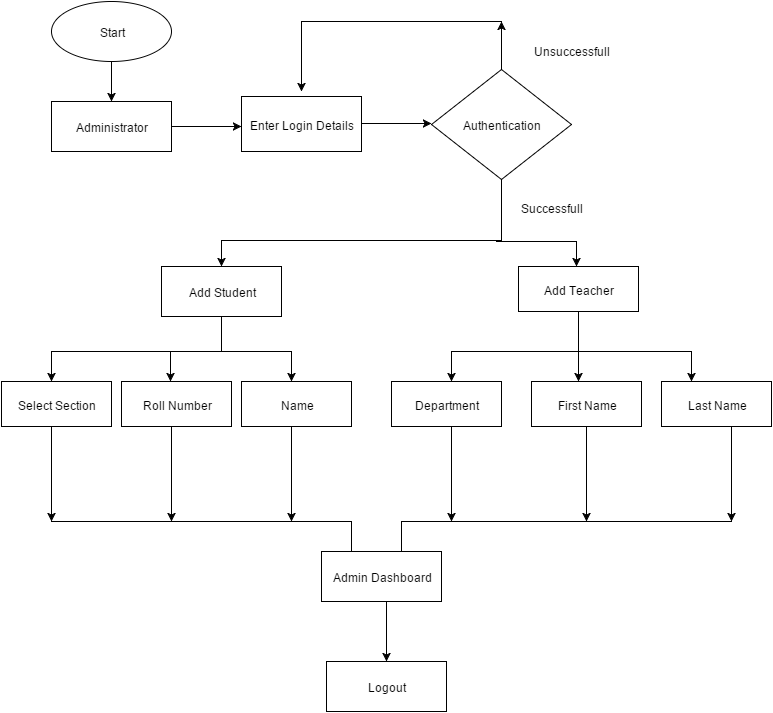
\includegraphics[scale=0.6]{images/addnew.png}
%\caption{Flow Chart For Adding New Teacher/Student}
%\end{figure}
\newpage
\image{0.5}{images/software.png}{Flow Chart For Working of System}
\newpage
\image{0.6}{images/addnew.png}{Flow Chart For Adding New Teacher/Student}

\newpage
\section{Database Design}
\image{0.4}{images/database.png}{Database Design}
\newpage
\section{Assumptions and Dependencies}
\subsection{Assumptions}
For Elearning System, main assumption was that this website may be viewed and even operated by literate person. Viewing the website is different than managing it. However it was not recommended to give access to uneducated people, but as the requirements specified by the client, the website must be designed in such a way that it should be so easy to manage that everyone can work on that.
\subsection{Dependencies}
However as such there is not any serious dependency of this system, but for viewer, it is recommended to it on modern browsers like FireFox and Google Chrome. However it also works with older browsers even with Internet Explorer. For user, it requires a Linux server. However it will also work on windows server if a WAMP/XAMPP server is installed.
As there is not hardware dependency of this website, i.e. it is viewable on all type of devices.

\chapter{Implementation}
\section{Introduction to PHP}
\begin{figure}[h]
\centering 
\includegraphics[scale=0.4]{images/php.png}
\caption{Php logo}
\end{figure}
\noindent PHP is an open source server-side scripting language designed for Web development to produce dynamic Web pages. It is one of the first developed server-side scripting languages to be embedded into an HTML source document rather than calling an external file to process data. The code is interpreted by a Web server with a PHP processor module which generates the resulting Web page. It also has evolved to include a command-line interface capability and can be used in standalone graphical applications.\\

\noindent PHP can be deployed on most Web servers and also as a standalone shell on almost every operating system and platform, free of charge. A competitor to Microsoft’s Active Server Pages (ASP) server-side script engine and similar languages, PHP is installed on more than 20 million Web sites and 1 million Web servers. Notable software that uses PHP includes Drupal, Joomla, MediaWiki, and WordPress. PHP is a general-purpose scripting language.\\

\noindent It is especially suited to server-side web development where PHP generally runs on a web server. Any PHP code in a requested file is executed by the PHP runtime, usually to create dynamic web page content or dynamic images used on Web sites or elsewhere. It can also be used for command-line scripting and client-side graphical user interface (GUI) applications. PHP can be deployed on most Web servers, many operating systems.
\subsection{Features of PHP}
\begin{itemize}
\item Http Authentication
\item Cookies and Sessions
\item Connection Handling
\item Designer-friendly 
\item Cross platform Compatibility 
\item Loosely typed Language
\item Open Source
\item Easy code
\end{itemize}



\section{MySQL Database Server}
\begin{figure}[h]
\centering 
\includegraphics[scale=0.2]{images/mysql.jpg}
\caption{Mysql logo}
\end{figure}
\noindent I used the Mysql database for my project. It is world''s most popular open source database It 
is a relational database management system (RDBMS) that runs as a server 
providing multi-user access to a number of databases. It is named after 
developer Michael Widenius's daughter, My. The SQL phrase stands for
Structured Query Language. MySQL is written in C and C++.\\

\noindent Free-software-open source projects that require a 
full-featured database management system
often use MySQL. MySQL is also used in many high-profile, large-scale World 
Wide Web products, including
Wikipedia, Google (though not for searches) and Facebook.\\

\noindent MySQL is a popular choice of database for use in web 
applications, and is a central component of the widely used LAMP web 
application software LAMP is an acronym for “Linux, Apache, MySQL, 
Perl/PHP/Python”. MySQL is used in some of the most frequently visited web sites 
on the Internet, including Flickr, Nokia.com, YouTube, Wikipedia, Google 
and Facebook.\\

\noindent One of the greatest advantage of Django is that it synchronises the 
database only with one command withouut having any need to send 
different queries for insertion, deletion, updation etc. There is a 
file named models.py which is used for purpose of creating database.
\subsection{Features of MySQL}
\begin{itemize}
\item MySQL is a database management system.
\item MySQL is a relational database management system.
\item MySQL software is Open Source.
\item The MySQL Database Server is very fast, reliable, and easy to 
use.
\item MySQL Server works in client/server or embedded systems.
\item A large amount of contributed MySQL software is available.
\end{itemize}
\subsection{Installation of MySQL}
MySql can be installed using following commands:\\

\hspace{4pt} \$ sudo apt-get install mysql-server\\

\hspace{4pt} \$ sudo apt-get install mysql-client


\section{Introduction to Bootstrap} 

\begin{figure}[h]
\centering 
\includegraphics[scale=0.3]{images/bootstrap.png}
\caption{Bootstrap logo}
\end{figure}
\subsection{What is Bootstrap}
\noindent Bootstrap is a powerful front-end framework for faster and easier web development. It includes HTML and CSS based design templates for common user interface components like Typography, Forms, Buttons, Tables, Navigations, Dropdowns, Alerts, Modals, Tabs, Accordion, Carousel and many other as well as optional JavaScript extensions.
Bootstrap also gives you ability to create responsive layout with much less efforts.
\subsection{Advantages of Bootstrap}
The biggest advantage of using Bootstrap is that it comes with free set of tools for creating flexible and responsive web layouts as well as common interface components.
Additionally, using the Bootstrap data APIs you can create advanced interface components like Scrollspy and Typeaheads without writing a single line of JavaScript.
Here are some more advantages, why one should opt for Bootstrap:
\begin{itemize}
\item Save lots of time.
\item Responsive features.
\item Consistent design .
\item Easy to use.
\item Compatible with browsers.
\item Open Source.
\item Consistency.
\item Comprehensive List Of Components
\item Leveraging Javascript Libraries.
\item Frequent Updates.
\end{itemize}
\subsection{Installation of Bootstrap}
Downloading of Bootstrap is a very easy proccess.
Type the commands in the terminal:\\

 \$ git clone https://github.com/twbs/bootstrap.git\\


\noindent This will clone the bootstrap files on your pc/laptop and later u can use these files in your project.


\section{Introduction to Apache Web Server}

\begin{figure}[h]
\centering
\includegraphics[scale=0.5]{images/apache.jpg}
\caption{Apache logo}
\end{figure}
\noindent Apache is a web server software notable for playing a key role in the initial 
growth of the World Wide Web. Apache is developed and maintained by an 
open community of developers under the auspices of the Apache Software 
Foundation. The application is available for a wide variety of operating 
systems, including Unix, FreeBSD, Linux, Solaris, Novell NetWare, Mac OS X, 
Microsoft Windows, OS/2, TPF, and eComStation. Released under the Apache 
License, Apache is open-source software.

\noindent The goal of this project is to provide a secure, efficient and extensible 
server that provides HTTP services in sync with the current HTTP standards.
\subsection{Features of Apache Server}
\begin{itemize}
\item Apache supports a variety of features, many implemented as compiled 
modules which extend the core functionality. These can range from 
server-side programming language support to authentication schemes. 
\item Apache features configurable error messages, DBMS-based 
authentication databases, and content negotiation. It is also supported 
by several graphical user interfaces (GUIs).
\item It supports password authentication and digital certificate 
authentication. Apache has a built in search engine and an HTML authorizing 
tool and supports FTP.
\end{itemize}

\subsection{Installation of Apache Server}
Apache web server can be installed using following commands:\\

\hspace{4pt} \$ sudo apt-get install apache2


\section{Introduction To Github}
\begin{figure}[h]
\centering 
\includegraphics[scale=0.27]{images/github.jpg}
\caption{Github logo}
\end{figure}
\noindent GitHub is a Git repository web-based hosting service which offers all of the functionality of Git as well as adding many of its own features. Unlike Git which is strictly a command-line tool, Github provides a web-based graphical interface and desktop as well as mobile integration. It also provides access control and several collaboration features such as wikis, task management, and bug tracking and feature requests for every project.\\

\noindent GitHub offers both paid plans for private repto handle everything from small to very large projects with speed and efficiency. ositories, and free accounts, which are usually used to host open source software projects. As of 2014, Github reports having over 3.4 million users, making it the largest code host in the world.\\

\noindent GitHub has become such a staple amongst the open-source development community that many developers have begun considering it a replacement for a conventional resume and some employers require applications to provide a link to and have an active contributing GitHub account in order to qualify for a job.\\\\

\section{What is Git?}
\begin{figure}[h]
\centering 
\includegraphics[scale=0.3]{images/git.jpg}
\caption{Git logo}
\end{figure}
\noindent Git is a distributed revision control and source code management (SCM) system with an emphasis on speed, data integrity, and support for distributed, non-linear workflows. Git was initially designed and developed by Linus Torvalds for Linux kernel development in 2005, and has since become the most widely adopted version control system for software development.\\

\noindent As with most other distributed revision control systems, and unlike most client–server systems, every Git working directory is a full-fledged repository with complete history and full version-tracking capabilities, independent of network access or a central server. Like the Linux kernel, Git is free and open source software distributed under the terms of the GNU General Public License version 2 to handle everything from small to very large projects with speed and efficiency.\\

\noindent Git is easy to learn and has a tiny footprint with lightning fast performance. It outclasses SCM tools like Subversion, CVS, Perforce, and ClearCase with features like cheap local branching, convenient staging areas, and multiple workflows.\\

\subsection{Installation of Git}

Installation of git is a very easy process.
The current git version is: 2.0.4.
Type the commands in the terminal:\\\\
\emph{
\$ sudo apt-get update\\\\
\$ sudo apt-get install git\\\\}
This will install the git on your pc or laptop.

\subsection{Various Git Commands}

Git is the open source distributed version control system that facilitates GitHub activities on your laptop or desktop. The commonly used Git command line instructions are:-\\

\subsection*{Create Repositories}
\addcontentsline{toc}{subsection}{Create Repositories}
Start a new repository or obtain from an exiting URL

\begin{description}

\item [\$ git init [ project-name]]\\
Creates a new local repository with the specified name
\item [\$ git clone [url]]\\
Downloads a project and its entire version history

\end{description}

\subsection*{Make Changes}
\addcontentsline{toc}{subsection}{Make Changes}
Review edits and craft a commit transaction

\begin{description}

\item [\$ git status] \leavevmode \\
Lists all new or modified files to be committed

\item [\$ git diff] \leavevmode \\
Shows file differences not yet staged

\item [\$ git add [file]]\\
Snapshots the file in preparation for versioning

\item [\$ git reset [file]]\\
Unstages the file, but preserve its contents

\item [\$ git commit -m "[descriptive message]"]\\
Records file snapshots permanently in version history

\end{description}

\subsection*{Group Changes}
\addcontentsline{toc}{subsection}{Group Changes}
Name a series of commits and combine completed efforts

\begin{description}

\item [\$ git branch] \leavevmode \\
Lists all local branches in the current repository

\item [\$ git branch [branch-name]]\\
Creates a new branch

\item [\$ git checkout [branch-name]]\\
Switches to the specified branch and updates the working directory

\item [\$ git merge [branch]]\\
Combines the specified branch’s history into the current branch

\item [\$ git branch -d [branch-name]]\\
Deletes the specified branch

\end{description}




%\section{Debconf}
%\input {input/debconf.tex}

\section{Introduction to \LaTeX}
\section{Introduction to \LaTeX}

\LaTeX, I have used this tool for preparing my six weeks training report and i found it excellent. So this time again i decided to use it for my report.
\LaTeX{} (pronounced /ˈleɪtɛk/, /ˈleɪtɛx/, /ˈlɑːtɛx/, or /ˈlɑːtɛk/) is a 
document markup language and document preparation system for the \TeX{} 
typesetting  program. Within the typesetting system, its name is styled 
as \LaTeX.

\image{0.9}{images/donald.png}{Donald Knuth, Inventor Of \TeX{} 
typesetting system}

\noindent Within the typesetting system, its name is styled as \LaTeX. The term 
\LaTeX{} refers only to the language in which documents are written, 
not to the editor used to write those documents. In order to create a 
document in \LaTeX, a .tex file must be created using some form of text 
editor. While most text editors can be used to create a \LaTeX{} document, 
a number of editors have been created specifically for working with \LaTeX.

\noindent \LaTeX{} is most widely used by mathematicians, scientists, 
engineers, philosophers, linguists, economists and other scholars in 
academia. As a primary or intermediate format, e.g., translating DocBook 
and other XML-based formats to PDF, \LaTeX{} is used because of the 
high quality of typesetting achievable by \TeX. The typesetting system 
offers programmable desktop publishing features and extensive facilities 
for automating most aspects of typesetting and desktop publishing, 
including numbering and cross-referencing, tables and figures, 
page layout and bibliographies.

\noindent \LaTeX{} is intended to provide a high-level language that
accesses the power of \TeX. \LaTeX{} essentially comprises a
collection of \TeX{} macros and a program to process \LaTeX documents. 
Because the \TeX{} formatting commands are very low-level, it is usually 
much simpler for end-users to use \LaTeX{}.


\section{Typesetting}
\LaTeX{} is based on the idea that authors should be able to focus on 
the content of what they are writing without being distracted by its 
visual presentation. In preparing a \LaTeX{} document, the author 
specifies the logical structure using familiar concepts such as 
chapter, section, table, figure, etc., and lets the \LaTeX{} system 
worry about the presentation of these structures. It therefore 
encourages the separation of layout from content while still allowing 
manual typesetting adjustments where needed. 

\begin{verbatim}
\documentclass[12pt]{article}
\usepackage{amsmath}
\title{\LaTeX}
\date{}
\begin{document}
  \maketitle 
  \LaTeX{} is a document preparation system 
  for the \TeX{} typesetting program.
   \par 
   $E=mc^2$
\end{document}
\end{verbatim}



\section{Introduction to Doxygen}
\begin{figure}[h]
\centering 
\includegraphics[scale=1]{images/doxygen.jpg}
\end{figure}
\noindent Doxygen is a documentation generator, a tool for writing software reference 
documentation. The documentation is written within code, and is thus 
relatively easy to keep up to date. Doxygen can cross reference 
documentation and code, so that the reader of a document can easily 
refer to the actual code.

\noindent Doxygen supports multiple programming languages, especially C++, C, 
C\#, Objective-C, Java, Python, IDL, VHDL, Fortran and PHP.[2] Doxygen
 is free software, released under the terms of the GNU General Public 
License.\\

\subsection{Features of Doxygen}
\begin{itemize}
\item Requires very little overhead from the writer of the documentation. 
Plain text will do, Markdown is support, and for more fancy or structured 
output HTML tags and/or some of doxygen's special commands can be used.
\item Cross platform: Works on Windows and many Unix flavors (including 
Linux and Mac OS X).
\item Comes with a GUI frontend (Doxywizard) to ease editing the options 
and run doxygen. The GUI is available on Windows, Linux, and Mac OS X.
\item Automatically generates class and collaboration diagrams in HTML 
(as clickable image maps) and $\mbox{\LaTeX}$ (as Encapsulated PostScript 
images).
\item Allows grouping of entities in modules and creating a hierarchy 
of modules.
\item Doxygen can generate a layout which you can use and edit to change 
the layout of each page.
\item Can cope with large projects easily.
\end{itemize}
\subsection{Installation of Doxygen}
Doxygen can be installed using following commands:\\

\hspace{4pt} \$ git clone https://github.com/doxygen/doxygen.git\\ 

\hspace{4pt} \$ cd doxygen\\

\hspace{4pt} \$ ./configure\\

\hspace{4pt} \$ make \\
\newpage



\newpage
\section{Implementation}
Implementation is the process of converting a new or revised system 
design into an operational one. At the present time there is no system 
as Imperial Finance which work online and provide information via web.
So this is the replacement of the manual financial system. In Imperial 
Finance most of the finance related task will be performed online.\\

{\bf Types of Implementation:}
\begin{enumerate}
\item Implementation of a computer system to replace a manual system.
\item Implementation of a new computer system to replace an existing one.
\item Implementation of a modified application to replace an existing one.\\
\end{enumerate} 

\hspace{0.0cm} {\bf Aspects of Implementation:}
\begin{enumerate}
\item Conversion
\item Post Implementation and review
\item Software maintenance
\end{enumerate}
\vskip 0.5cm
\subsection{Implementation of the Project }
Elearning System is the implementation of the new system to replace manual one. Working manually is very time consuming and irritating. The project 
implementation of starts with the Administrator. Administrator will be the super user of the application who will configure system information. There will be a different interface for the Students and Teachers from where they can manage and view the required information.\\

\noindent It is a web based application, so it is distributed and data centric. 
In this application, MySQL database is used to store data related to 
Students and Teachers. Since database is on 
Server, so any number of users can work simultaneously and can share 
their data with each other.
\subsection{Conversion Plan}
Conversion is the process of changing from one system to another. This 
plan involves:
\begin{enumerate}
\item Creating computer-compatible files.
\item Training the operating staff.
\item Installing terminals and hardware.
\end{enumerate}

\subsection{Conversion Processes}
\begin{enumerate}
\item File Conversion.
\item  Data Entry.
\item User Training.
\end{enumerate}
\vskip 0.5cm
\subsection{Elements of User training}
\begin{enumerate}
\item The initial training period.
\item At the time of Installation.
\item If required, during Maintenance Phase.
\end{enumerate}

\section{Post-Implementation and Software Maintenance}
Implementation review is an evaluation of a system in terms of the 
extent to which the system accomplishes stated objectives and actual 
project costs exceeds initial estimates.
\subsection{Review Plan}
An overall plan covers following aspects:
\begin{enumerate}
\item Administrative plan.
\item Personnel requirements plan.
\item Hardware plan.
\item Documentation review plan.
\end{enumerate}
\vskip 0.5cm
After the implementation of this project, the team will see the post 
implementation phase. If there will be any concerns, those will be 
solved based on the user feedback.
\subsection{Maintenance}
In order for a software system to remain useful in its environment it 
may be necessary to carry out a wide range of maintenance activities 
upon it. There are bugs to fix, enhancement to add and optimization to 
make, changes has to be done in older version to make it application 
for current use of current version to cater the need of future. 
Maintenance can be of three types:\\
\begin{enumerate}
\item {\bf{Corrective Maintenance}}: Changes necessitated by actual errors 
(defects or residual "bugs") in a system are termed corrective 
maintenance. These defects manifest themselves when the system does not
operate as it was designed or advertised to do. A defect or “bug” can 
result from design errors, logic errors and coding errors. Design errors 
occur when for example changes made to the software are incorrect, 
incomplete, wrongly communicated or the change request misunderstood. 
In the event of a system failure due to an error, actions are taken to 
restore operation of the software system. The approach here is to locate 
the original specifications in order to determine what the system was 
originally designed to do.
\item {\bf{Adaptive Maintenance}}: Any effort that is initiated as a result of 
changes in the environment in which a software system must operate is 
termed adaptive change. Adaptive change is a change driven by the need
to accommodate modifications in the environment of the software system, 
without which the system would become increasingly less useful until it 
became obsolete. The term environment in this context refers to all the 
conditions and influences which act from outside upon the system, for 
example business rules, government policies, work patterns, software 
and hardware operating platforms. A change to the whole or part of this 
environment will warrant a corresponding modification of the software.
\item {\bf{Perfective Maintenance}}: This is actually the most common type of 
maintenance encompassing enhancements both to the function and the 
efficiency of the code and includes all changes, insertions, deletions, 
modifications, extensions, and enhancements made to a system to meet 
the evolving and/or expanding needs of the user. A successful piece of 
software tends to be subjected to a succession of changes resulting in 
an increase in its requirements. This is based on the premise that as 
the software becomes useful, the users tend to experiment with new 
cases beyond the scope for which it was initially developed. Expansion 
in requirements can take the form of enhancement of existing system 
functionality or improvement in computational efficiency. Though 
efforts have been made to develop error free systems, but no system is 
perfect, room for improvement is always there. Thus proper documentation 
for the system has been done so that it will be easy to handle any 
breakdown or any other type of system maintenance activity.

\end{enumerate}

\section{Testing}
Project testing is an investigation conducted to determine the quality of the project and the services provided by the project. Testing is the process of analyzing a project to detect the differences between existing and required conditions (that is defects/errors/bugs) and to evaluate the features of the project. After complete development of the project it is mandatory to test the project. The main motive of the project testing is to identify whether project is able to meet user
requirements or not. To know the better performance of project we have to develop various Test Cases. Now, designing good test cases is a complex art. The complexity comes from three sources
\begin{itemize}
\item Test cases help us discover information. Different types of tests are more effective for different classes of information.
\item Test cases can be good in a variety of ways. No test case will be good in all of them.
\item Our tend to create test cases according to certain testing styles, such as domain testing or risk-based testing. Good domain tests are different from good risk-based tests.
\end{itemize}
\subsection{Unit Testing}
Unit testing is undertaken after a module has been coded and successfully reviewed. Unit testing (or module testing) is the testing of different units (or modules) of a system in isolation. I have done unit testing for my project. Before combining all modules i have tested the modules independently, and no errors were reported during testing.
\subsection{Integration Testing}
In this type of testing I have used Big Bang Approach, where all the modules
making up a system are integrated in a single step. In simple words, all the modules of the system are simply put together and tested. However, this technique is practicable only for very small systems. The main problem with this approach is that once an error is found during the integration testing, it is very difficult to localize the error as the error may potentially belong to any of the modules being integrated. Therefore, debugging errors reported during big bang integration testing are very expensive to fix. During this testing no errors were reported and the system worked fine.
\subsection{System Testing}
System tests are designed to validate a fully developed system to assure that it meets its requirements. I have performed this testing to the software and all the requirements that were kept in mind before the development of this system are fulfilled. The system as whole worked as expected and also no errors or problems were reported.
\newpage
\section{Project Screenshots}
\image{0.31}{images/home.png}{Home Page}
\image{0.37}{images/classcalender}{Class Calender}
\image{0.5}{images/signupstudent.png}{Student Signup}
\image{0.5}{images/signupteacher.png}{Teacher Signup}
\image{0.43}{images/studentdashboard.png}{Student Dashboard}
\image{0.4}{images/teacherdashboard.png}{Teacher Dashboard}
\image{0.4}{images/addassignment.png}{Add Assignment}
\image{0.4}{images/submitassignment.png}{Submit Assignment}
\image{0.5}{images/sendmessage.png}{Send Message}
\image{0.5}{images/viewprogress.png}{View Progress}
\image{0.37}{images/admindashboard.png}{Admin Dashboard}
\image{0.45}{images/addstudent.png}{Add New Student}
\newpage

\chapter{Prject Legacy}
\input{input/legacy.tex}
\input{input/bibliography.tex}
\end{document}

